\documentclass[../main.tex]{subfiles}
\usepackage{tikz}
\usepackage{xcolor}
\begin{document}

Chương này trình bày các kiến thức nền tảng phục vụ cho nghiên cứu của đồ án, bao gồm khái niệm về công nghệ vận hành (OT), hệ thống điều khiển công nghiệp (ICS), bộ điều khiển logic khả trình (PLC), mô hình kiến trúc mạng Purdue, giao thức Siemens S7comm và hệ thống phát hiện xâm nhập (IDS). Nội dung chương là cơ sở để hiểu bối cảnh vận hành, điểm yếu bảo mật và hướng tiếp cận phát hiện tấn công trên giao thức S7comm trong các chương tiếp theo.

\section{Tổng quan về hệ thống OT và ICS}
\label{sec:ot-ics}

Mọi công nghệ để vận hành nhà máy vật lý được gọi là OT (\textit{Operational Technology}), bao gồm:

\begin{itemize}
    \item Công nghệ giám sát và quản lý phụ trợ như BMS (\textit{Building Management Systems}) để điều khiển điều hòa (HVAC), chiếu sáng, phòng cháy chữa cháy; EMS (\textit{Energy Management Systems}) để quản lý năng lượng tiêu thụ.
    \item Công nghệ bảo trì như EAM (\textit{Enterprise Asset Management}) để theo dõi tình trạng thiết bị.
    \item Công nghệ giao thông và điều khiển vận hành hiện trường.
    \item Công nghệ điều khiển ICS (\textit{Industrial Control Systems}) là cách điều khiển và giám sát các quy trình công nghiệp. Trong hệ thống ICS bao gồm các thành phần chính sau:
\end{itemize}

\begin{center}
    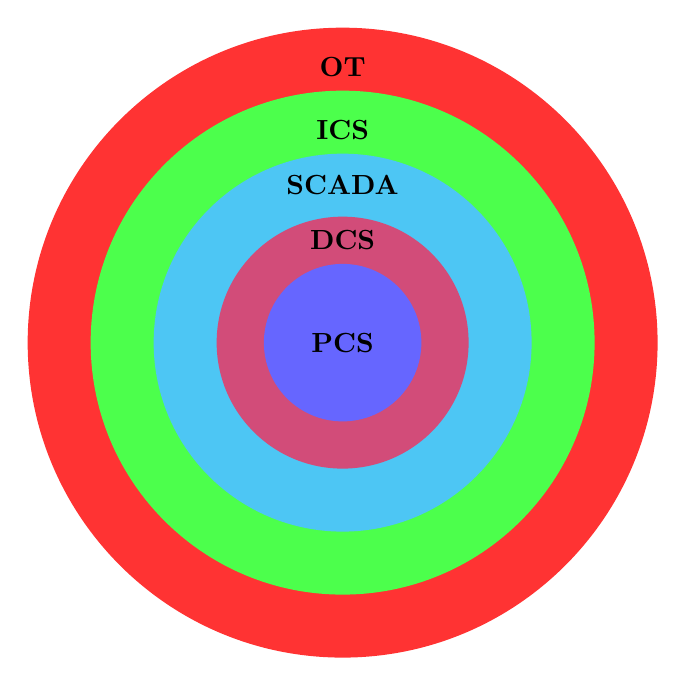
\begin{tikzpicture}
    
    % Vòng ngoài cùng (OT)
    \fill[red!80] (0,0) circle (4);
    
    % ICS
    \fill[green!70] (0,0) circle (3.2);
    
    % SCADA
    \fill[cyan!70] (0,0) circle (2.4);
    
    % DCS
    \fill[purple!70] (0,0) circle (1.6);
    
    % PCS
    \fill[blue!60] (0,0) circle (1);
    
    % Text labels
    \node at (0,3.5) {\textbf{OT}};
    \node at (0,2.7) {\textbf{ICS}};
    \node at (0,2.0) {\textbf{SCADA}};
    \node at (0,1.3) {\textbf{DCS}};
    \node at (0,0) {\textbf{PCS}};
    
    \end{tikzpicture}
    \end{center}

\begin{itemize}
    \item \textbf{Industrial Control Systems (ICS)}: hoạt động điều khiển các quy trình công nghiệp nói chung.
    \item \textbf{Supervisory Control and Data Acquisition (SCADA)}: cung cấp khả năng giám sát, phân tích thời gian thực và quản lý ở mức cao cho các thiết bị trải rộng trên \textbf{nhiều vùng địa lý} tại một trung tâm chỉ huy duy nhất.
    
    \begin{figure}[H]
    \centering
    
\includegraphics[width=0.55\textwidth]{Figure/SCADA.png}
    \caption{Ví dụ một hệ thống SCADA}
    \label{fig:scada}
    \end{figure}


    Hệ thống SCADA quản lý và giám sát 3 nhà máy tại 3 khu vực địa lý khác nhau Texas, North Dakota, Alaska. SCADA Control Center bao gồm Control Servers, HMI, Historian, Engineering Workstation, Communication Infrastructure, nằm tại Supervisory Zone

    \item \textbf{Distributed Control Systems (DCS)}: tập trung vào việc điều khiển các quá trình công nghiệp phức tạp, 
    liên tục và cần sự phối hợp của nhiều bộ điều khiển đơn lẻ, được kết nối với nhau bằng một bộ điều khiển trung tâm để phối hợp hoạt động. Việc tách ra làm các bộ điều khiển đơn lẻ cho từng process cụ thể trong process tổng thể giúp các bộ điều khiển ở gần với process mà nó điều khiển hơn, viết logic đơn giản hơn, giảm độ trễ và bảo trì. Tuy nhiên, các bộ điều khiển này đều nằm trong cùng một khu vực địa lý. DCS thường được sử dụng trong các nhà máy lớn và phức tạp, nơi có hàng ngàn thông số cần được phối hợp và điều khiển đồng thời với độ tin cậy cao

    \item \textbf{Process Control Systems (PCS)}: khái niệm chung chỉ một hệ con (\textit{subsystem}) thực hiện chuyên biệt một tác vụ/chức năng cụ thể trong toàn bộ quá trình sản xuất. Một ICS có thể bao gồm hàng trăm PCS.

    \begin{figure}[H]
    \centering
    
\includegraphics[width=0.55\textwidth]{Figure/DCS.png}
    \caption{Ví dụ về một hệ thống DCS triển khai tại một nhà máy}
    \label{fig:dcs}
    \end{figure}

    Nhà máy đặt tại Alaska trong số ba nhà máy được giám sát bởi SCADA phía trên sử dụng DCS, bao gồm nhiều bộ điều khiển đơn 
    lẻ (Local Control Unit), mỗi bộ điều khiển này sẽ thực hiện một chức năng cụ thể trong dây chuyền sản xuất (PCS). Trong một PCS bao gồm các thành phần sau:

    \begin{itemize}
        \item \textbf{Field Devices}: chuyển đổi qua lại giữa tín hiệu từ các quy trình vật lý và tín hiệu điện tử, gồm:
        \begin{itemize}
            \item \textbf{Sensors}: đo lường các thông số vật lý như nhiệt độ, áp suất, lưu lượng, độ ẩm\ldots\ và chuyển thành tín hiệu điện tử đầu vào.
            \item \textbf{Actuators}: nhận tín hiệu điện tử đầu ra để điều khiển thiết bị thực thi các quy trình vật lý như van, bơm, động cơ\ldots
        \end{itemize}

        \item \textbf{Field Controller}: bộ điều khiển hiện trường, gồm:
        \begin{itemize}
            \item \textbf{PLC} (\textit{Programmable Logic Controller}): thiết bị có khả năng lập trình; nhận tín hiệu đầu vào $\rightarrow$ xử lý các phép toán logic đã lập trình sẵn $\rightarrow$ xuất tín hiệu đầu ra. Đồng thời gửi dữ liệu quá trình về HMI và nhận lệnh điều khiển từ HMI.

            \item \textbf{IED} (\textit{Intelligent Electronic Device}): tương tự PLC nhưng chuyên điều khiển thiết bị mạch điện như rơle bảo vệ, \textit{on-load tap changer}, máy cắt (\textit{circuit breaker}). IED thường chạy độc lập chương trình đã lập trình sẵn hơn là nhận lệnh điều khiển trực tiếp từ HMI.

            \item \textbf{RTU} (\textit{Remote Terminal Unit}): tương tự PLC nhưng tập trung truyền tải dữ liệu \textit{telemetry} từ xa về trung tâm điều khiển; thường được trang bị các chuẩn giao tiếp xa, không dây mạnh mẽ hơn PLC như RF, vệ tinh, cellular\ldots

            \item \textbf{PAC} (\textit{Programmable Automation Controller}): mở rộng khả năng của PLC, gần với mô hình PC kết hợp PLC; hỗ trợ lập trình bằng năm ngôn ngữ IEC~61131-3 và thêm C/C++. PAC hỗ trợ nhiều module I/O hơn, xử lý logic phức tạp hơn, tích hợp xử lý dữ liệu và kết nối cơ sở dữ liệu, thường dùng cho điều khiển và giám sát đa miền (\textit{multi-domain}).
        \end{itemize}

        \item \textbf{HMI} (\textit{Human Machine Interface}): giao diện giữa con người và máy móc. Chiều Human $\rightarrow$ Machine chuyển tương tác của người vận hành thành tín hiệu mà máy hiểu được; chiều Machine $\rightarrow$ Human chuyển tín hiệu thành biểu tượng, đồ thị như trạng thái (\textit{status}), báo động (\textit{alarms}) và thông báo (\textit{notifications}).
    \end{itemize}

    \item \textbf{SIS (Safety Instrumented System)}: hệ thống điều khiển giống PLC nhưng được triển khai \textbf{độc lập, cách ly} với hệ thống điều khiển chính để tạo thêm một lớp an toàn bổ sung trong trường hợp 
    hệ thống điều khiển chính bị Lỗi

    \begin{figure}[H]
    \centering
    
\includegraphics[width=0.55\textwidth]{Figure/SIS.png}
    \caption{Ví dụ hệ thống SIS}
    \label{fig:sis}
    \end{figure}

    SIS Controller cũng giống PLC/RTU nhưng sử dụng 2 Gauges Level Sensors, 2 Valve Actuator của riêng 
    nó để điều khiển mực nước trong bể chứa. Dù cho PLC có hỏng hay Sensor chính gặp vấn đề thì vẫn còn SIS dự 
    phòng để đảm bảo an toàn.

    \item \textbf{EMS (Energy Management System)}: hệ thống quản lý năng lượng, giúp tối ưu hóa việc sử dụng, truyền tải và phân phối năng lượng để nhà máy vận hành hiệu quả và không làm quá tải lưới điện.
\end{itemize}

\section{Bộ điều khiển logic khả trình (PLC)}
\label{sec:plc}

\subsection{Khái niệm PLC}

PLC là tên viết tắt của \textbf{Programmable Logic Controller} là bộ điều khiển logic khả trình hay bộ điều khiển logic có khả năng lập trình. PLC về bản chất giống mới một chiếc PC chạy chương trình do lập trình viên viết ra. Điểm khác biệt duy nhất nằm ở chất lượng phần cứng đặc biệt tốt, nhỏ gọn để chịu được môi trường đặc thù nhiều rung động, nhiệt độ cao, bụi bẩn, nhiễu điện từ, hoạt động liên tục 24/7 trong nhiều năm của các nhà máy sản xuất.

Trước khi PLC ra đời, việc điều khiển các quy trình này thường được thực hiện bằng hàng trăm, thậm chí hàng nghìn rơ le (relay), bộ định thời (timer), và bộ đếm (counter) cơ điện. Hệ thống này rất cồng kềnh, phức tạp, khó khăn trong việc sửa đổi logic điều khiển. Sự ra đời của PLC vào cuối những năm 1960 bởi \textbf{Richard E. Morley} được xem là một cuộc cách mạng, thay thế hoàn toàn các hệ thống điều khiển bằng rơ le truyền thống. Điểm đặc biệt của PLC so với các hệ thống điều khiển cứng bằng rơ le là logic điều khiển có thể dễ dàng thay đổi bằng cách sửa đổi chương trình phần mềm mà không cần phải thay đổi phần cứng hay đi lại dây phức tạp.

Thị trường PLC toàn cầu được thống trị bởi một số ít nhà sản xuất lớn, mỗi hãng có dòng sản phẩm, 
phần mềm lập trình và hệ sinh thái riêng. Việc lựa chọn PLC thường phụ thuộc vào kinh nghiệm đội 
ngũ kỹ thuật, tính sẵn có của thiết bị và hỗ trợ kỹ thuật có sẵn tại nhà máy.

\begin{table}[H]
    \centering
    \caption{Các nhà sản xuất PLC tiêu biểu}
    \label{tab:plc-manufacturers}
    \begin{tabular}{|p{3.2cm}|p{1.8cm}|p{4.2cm}|p{3.5cm}|}
        \hline
        \textbf{Tên} & \textbf{Quốc gia} & \textbf{Các dòng máy phổ biến} & \textbf{Phần mềm lập trình} \\
        \hline
        Siemens & Đức & LOGO!, Simatic S7-200 SMART, S7-300, S7-400, S7-1200, S7-1500 & TIA Portal \\
        \hline
        Rockwell Automation / Allen-Bradley & Mỹ & MicroLogix, CompactLogix, ControlLogix & RSLogix 5000, Studio 5000 \\
        \hline
        Mitsubishi Electric & Nhật Bản & FX, Q, L, iQ-R/F series & GX Works2, GX Works3 \\
        \hline
        Omron & Nhật Bản & CP1, CJ2, NX/NJ series & CX-One \\
        \hline
        Schneider Electric & Pháp & Modicon M221, M340, M580 & EcoStruxure Control Expert \\
        \hline
    \end{tabular}
\end{table}

Ngoài ra còn các nhà sản xuất khác như Delta (Đài Loan), Keyence (Nhật Bản) và LS Electric (Hàn Quốc)\ldots

\subsection{Cấu tạo PLC}

\begin{figure}[H]
    \centering
    
\includegraphics[width=0.85\textwidth]{Figure/PLC_components.png}
    \caption{Các thành phần chính của PLC}
    \label{fig:plc-components}
\end{figure}

\subsubsection{Bộ xử lý trung tâm (CPU)}

\textbf{Bộ xử lý trung tâm CPU} (\textit{Central Processing Unit}) được coi là bộ não của PLC. Khác với CPU
 của máy tính thông thường hoạt động đa nhiệm và theo sự kiện (\textit{event-driven}), CPU của PLC hoạt 
 động theo chu kỳ quét (\textit{scan cycle}, thường tính bằng miligiây) và thực hiện tuần tự các lệnh trong chương trình. Một chu trình quét điển hình gồm 3 bước chính:

\begin{enumerate}
    \item \textbf{Đọc đầu vào (Input Scan)}: CPU kiểm tra trạng thái cảm biến, nút nhấn kết nối module đầu vào và chép dữ liệu vào Bảng ảnh đầu vào (\textit{Input Image Table} -- PII), đảm bảo CPU có bản chụp nhất quán về trạng thái đầu vào.
    \item \textbf{Thực thi chương trình (Program Execution)}: CPU chạy chương trình đã nạp sẵn để xử lý logic, số học và các lệnh điều khiển dựa trên đầu vào nhận được.
    \item \textbf{Cập nhật đầu ra (Output Scan)}: Sau khi tính toán xong, CPU cập nhật giá trị vào Bảng ảnh đầu ra (\textit{Output Image Table} -- PIQ), sau đó ghi ra module đầu ra để điều khiển các thiết bị chấp hành (động cơ, van, đèn\ldots).
    \item \textbf{Lặp lại chu trình quét}.
\end{enumerate}

Ngoài thực thi logic chính, CPU còn quản lý chuẩn đoán lỗi và giao tiếp với PLC hoặc hệ thống khác. CPU của PLC 
thường được thiết kế dựa trên các kiến trúc Intel X86, PowerPC, ARM, MIPS.


\subsubsection{Module đầu vào và đầu ra}

\textbf{Module đầu vào (Input Modules)} nhận tín hiệu từ thiết bị hiện trường và chuyển thành tín hiệu logic mà CPU hiểu được. Có hai loại chính:
\begin{itemize}
    \item Module đầu vào số (DI -- \textit{Digital Input Module}): nhận tín hiệu ON/OFF.
    \item Module đầu vào tương tự (AI -- \textit{Analog Input Module}): nhận tín hiệu liên tục.
\end{itemize}

Số lượng I/O mà PLC quản lý phản ánh khả năng xử lý và quy mô ứng dụng:

\begin{table}[htbp]
    \centering
    \caption{Phân loại PLC theo số lượng điểm I/O}
    \label{tab:plc-io-scale}
    \begin{tabular}{|l|c|}
        \hline
        \textbf{Loại PLC} & \textbf{Số lượng I/O} \\
        \hline
        Micro PLC & dưới 32--64 điểm I/O \\
        \hline
        Small PLC & 64 đến vài trăm điểm I/O \\
        \hline
        Medium PLC & vài trăm đến khoảng 1000--2000 điểm I/O \\
        \hline
        Large PLC & hàng nghìn, hàng chục nghìn điểm I/O \\
        \hline
    \end{tabular}
\end{table}

\textbf{Module đầu ra (Output Modules)} nhận lệnh từ CPU và chuyển thành tín hiệu điều khiển thiết bị chấp hành. Tương tự có:

\begin{itemize}
    \item Module đầu ra số (DO) xuất tín hiệu ON/OFF (Relay, Transistor, Triac)
    \item Module đầu ra tương tự (AO) xuất tín hiệu liên tục.
\end{itemize} 


\subsubsection{Bộ nhớ}

Trong PLC bao gồm các loại bộ nhớ sau:

\begin{itemize}
    \item \textbf{Read-only Memory (ROM)}: Chứa firmware, OS của PLC. Do phần này không thay đổi trong quá trình hoạt động của PLC nên chỉ cần Read. OS của PLC thường riêng biệt để tối ưu cho môi trường Real-time (RTOS Real-time Operating System), điển hình như VxWorks, Windows CE, Neutrino \& RTOS.
    \item \textbf{Random Access Memory (RAM)}: Chứa dữ liệu tạm thời như trạng thái I/O, timer, counter, biến nội bộ. Mất dữ liệu khi mất điện.  Các vùng nhớ quan trọng~\cite{snap7_sharp7}:

    \begin{table}[H]
        \centering
        \caption{Các vùng nhớ RAM trong PLC (theo ký hiệu Siemens)}
        \label{tab:plc-memory}
        \begin{tabular}{|l|c|p{7.5cm}|}
            \hline
            \textbf{Vùng nhớ} & \textbf{Ký hiệu} & \textbf{Ý nghĩa} \\
            \hline
            Input & I hoặc E & Lưu trạng thái của các cổng vào vật lý (nút nhấn, công tắc hành trình). PLC đọc từ phần cứng và chép vào đây ở đầu chu kỳ quét. \\
            \hline
            Output & Q hoặc A & Lưu trạng thái mong muốn của các thiết bị chấp hành (motor, đèn, van). Cuối chu kỳ quét, dữ liệu từ đây sẽ được đẩy ra phần cứng. \\
            \hline
            Memory/Merker & M & Vùng nhớ trung gian toàn cục của PLC, giống global variables trong IT. Nó dùng để lưu các trạng thái trung gian của thuật toán mà không xuất trực tiếp ra ngoài phần cứng. \\
            \hline
            Data Block & DB & Khối dữ liệu người dùng; lưu setpoint, giới hạn nhiệt độ/áp suất, mật khẩu\ldots \\
            \hline
            Local data & L & Lưu trữ các biến cục bộ trong các khối chương trình \\
            \hline
            Timer & T hoặc \%T & Bộ đếm thời gian. \\
            \hline
            Counter & C hoặc \%C & Bộ đếm sự kiện. \\
            \hline
        \end{tabular}
    \end{table}


    \item \textbf{Electrically Erasable Programmable Read-Only Memory (EEPROM)}: Thao tác với dữ liệu ở cấp độ Byte. Không mất dữ liệu khi mất điện. Thường dùng cho lưu trữ chương trình và dữ liệu cấu hình của PLC.
    \item \textbf{Flash Memory}: Giống EEPROM nhưng thao tác với dữ liệu ở cấp độ Block. Dung lượng lớn, nhanh và rẻ hơn.
\end{itemize}

\subsubsection{Các thành phần khác}

\textbf{Bộ nguồn (Power Supply Unit)} cung cấp điện áp ổn định cho các thành phần PLC, dự trữ năng lượng (UPS) để bảo vệ các thiết bị khi mất nguồn điện đột ngột.

\textbf{Cổng truyền thông (Communication Processor)} cho phép PLC giao tiếp với máy trạm nạp chương trình, HMI, SCADA, PLC khác hoặc hệ thống quản lý dữ liệu. PLC có thể
giao tiếp qua các loại Serial cũ như RS-232, RS-485 hoặc cổng Ethernet RJ45 hiện đại.


Các thành phần này có thể được tách ra thành từng module vật lý khác nhau và kết nối lại với nhau thành một PLC hoàn chỉnh thông qua bus hệ thống (\textit{Modular PLC}) (Modular PLC) hoặc được tích hợp sẵn trong một khối duy nhất (\textit{Compact PLC} hay \textit{Brick PLC}).

\begin{figure}[H]
    \centering
    \begin{subfigure}[t]{0.45\textwidth}
        \centering
        
\includegraphics[width=\textwidth]{Compact_PLC_type.png}
        \caption{LOGO! Siemens -- Compact PLC}
    \end{subfigure}
    \hfill
    \begin{subfigure}[t]{0.45\textwidth}
        \centering
        
\includegraphics[width=\textwidth]{Modular_PLC_type.png}
        \caption{Siemens S7-1200 -- Modular PLC}
    \end{subfigure}
    \caption{Hai dạng PLC: Compact và Modular}
    \label{fig:plc-types}
\end{figure}

Với PLC dạng module, các thành phần được gắn theo \textit{slot} trên \textit{rack} của tủ điện:

\begin{figure}[H]
    \centering
    
\includegraphics[width=0.85\textwidth]{Figure/PLC_rack.png}
    \caption{Trong phần mềm lập trình Tia Portal sẽ cần chỉ định rack và slot của module truyền thông của PLC, như ví dụ trong ảnh là rack 0, slot 1 để có thể kết nối tới đúng PLC}
    \label{fig:plc-rack}
\end{figure}

\subsection{Ngôn ngữ lập trình PLC}

Chương trình điều khiển PLC được viết bằng 5 ngôn ngữ lập trình theo chuẩn \textbf{IEC 61131-3}:

\begin{figure}[htbp]
    \centering
    
\includegraphics[width=0.85\textwidth]{Figure/Code_PLC.png}
    \caption{Năm ngôn ngữ lập trình PLC theo IEC 61131-3}
    \label{fig:plc-languages}
\end{figure}

\begin{enumerate}
    \item \textbf{Ladder Diagram (LD)}: ngôn ngữ đồ họa dạng mạch rơle, bao gồm 2 thanh dọc (Bus Bar) đại diện cho dây nóng và 
    dây trung tính, nối giữa 2 thanh dọc này là các thanh 
    ngang (rung) đại diện cho các dòng logic điều khiển bao gồm các đầu
     vào, các biến đổi logic nối với đầu ra và các tiếp điểm (Contacts) và cuộn dây (Coils). PLC sẽ scan các rungs từ trên xuống dưới, 
     mỗi rungs scan logic từ trái qua phải. Mỗi chu kỳ scan ~50-60ms. Đây là ngôn ngữ phổ biến nhất được sử dụng bởi các lỹ sư lập trình PLC do nó 
     có tư duy thiết kế giống với dạng mạch điện tử.
    
    \begin{figure}[H]
        \centering
        
\includegraphics[width=0.7\textwidth]{Figure/Ladder.png}
        \caption{Ví dụ một chương trình mạch tự duy trì băng ngôn ngữ Ladder}
        \label{fig:ld-example}
    \end{figure}

    \item \textbf{Function Block Diagram (FBD)}:  Logic bằng block function. Các khối hình chữ nhật với đầu vào bên trái và đầu ra bên phải, được nối với nhau bằng các đường kẻ (dây tín hiệu). Cho phép xây dựng các ứng dụng điều khiển phức tạp một cách trực quan. 

    \begin{figure}[H]
        \centering
        
\includegraphics[width=0.7\textwidth]{FBD_code.png}
        \caption{Ví dụ mã FBD}
        \label{fig:fbd-example}
    \end{figure}

    \item \textbf{Sequential Function Chart (SFC)}: Giống như một lưu đồ (flowchart) gồm các bước (Steps) và các điều kiện chuyển bước (Transitions). Sử dụng cho quy trình phức tạp và tuần tự

    \begin{figure}[H]
        \centering
        
\includegraphics[width=0.7\textwidth]{SFC_code.png}
        \caption{Ví dụ mã SFC}
        \label{fig:sfc-example}
    \end{figure}

    \item \textbf{Structured Text (ST)}: Là các dòng mã thuần văn bản, có dạng gần giống C / Pascal.  Phù hợp các lập trình viên code cho các ứng dụng phức tạp, có nhiều tính toán và xử lý dữ liệu, dùng  các cấu trúc như \texttt{IF...THEN}, \texttt{FOR}, \texttt{WHILE}

\begin{quote}
\small\ttfamily
IF Input1 THEN\\
\quad Output1 := NOT Output1;\\
END\_IF;
\end{quote}

    \item \textbf{Instruction List (IL)}: Ngôn ngữ cấp thấp, tương tự như Assembly. Tức gồm một danh sách các lệnh viết tắt theo cột dọc. Đòi hỏi lập trình viên có kiến thức chuyên sâu về PLC và kiến trúc máy tính, sử dụng cho các ứng dụng cần tốc độ xử lý cao và có yêu cầu về hiệu suất. Tuy nhiên không còn được khuyến khích sử dụng bởi các nhà sản xuất.

\begin{quote}
\small\ttfamily
LD Input1 \hfill\textit{(Load Input 1)}\\
AND Input2 \hfill\textit{(And với Input 2)}\\
ST Output1 \hfill\textit{(Store vào Output 1)}
\end{quote}
\end{enumerate}

\section{Mô hình Purdue}
\label{sec:purdue}

Mô hình Purdue (\textit{Purdue Enterprise Reference Architecture} -- PERA) là 
mô hình tiêu chuẩn để phân chia các lớp mạng trong môi trường ICS/OT.

\begin{figure}[H]
    \centering
    
\includegraphics[width=0.85\textwidth]{Figure/Purdue.png}
    \caption{Mô hình phân vùng mạng Purdue}
    \label{fig:purdue-overview}
\end{figure}

Kiến trúc này hiển thị khái niệm phân đoạn mạng giúp tách vùng của Mạng ICS (OT) khỏi Vùng của Mạng doanh nghiệp (IT). Nó cũng cho thấy sự phụ thuộc lẫn nhau và tương tác giữa các thành phần chính ở cấp độ 0 đến 5. Mô hình này được áp dụng từ IEC 62443, một bộ tiêu chuẩn về An ninh mạng trong các mạng công nghiệp.

Bảng~\ref{tab:purdue-layers-ot} và Bảng~\ref{tab:purdue-layers-it} mô tả chi tiết từng tầng, thiết bị điển hình và ví dụ thực tế tại nhà máy VinFast Hải Phòng (VF HP).

\begin{table}[H]
    \centering
    \caption{Phân tầng mạng Purdue --- vùng OT (tầng 0--2)}
    \label{tab:purdue-layers-ot}
    \footnotesize
    \renewcommand{\arraystretch}{1.25}
    \begin{tabular}{|>{\raggedright\arraybackslash}p{2.1cm}|>{\raggedright\arraybackslash}p{4.3cm}|>{\raggedright\arraybackslash}p{7.2cm}|}
        \hline
        \textbf{Tầng} & \textbf{Mô tả} & \textbf{Thiết bị} \\
        \hline
        0 --- \textit{Physical Layer} &
        Nơi tín hiệu điện/quang được chuyển thành quy trình vật lý (với Actuator) hoặc theo chiều ngược lại (với Sensor). &
        \textbf{Sensor}: đo các thông số vật lý như nhiệt độ, hình ảnh\ldots\ Ví dụ tại VF HP dùng cảm biến máy ảnh Zeiss kiểm tra thân vỏ xe.
        \par\vspace{0.3em}
        \textbf{Actuator}: van, cánh tay robot\ldots\ Ví dụ tại VF HP dùng cánh tay robot ABB kết hợp súng hàn ISI Welding Gun.
        \par\vspace{0.3em}
        
\includegraphics[width=0.6\linewidth]{Figure/ABB.png} \\
        \hline
        1 --- \textit{Controller Layer} &
        Chứa các bộ điều khiển nhận tín hiệu từ Sensor $\rightarrow$ xử lý logic điều khiển $\rightarrow$ xuất tín hiệu điều khiển cho Actuator. &
        PLC, RTU. Ví dụ tại VF HP, xưởng BODY sử dụng 98 PLC S7-1500 điều khiển toàn bộ dây chuyền. Bản thân các PLC này không điều khiển trực tiếp các cánh tay robot ABB mà sẽ gửi task chỉ là một số thứ tự xuống ABB robot controller. Các controller này chứa các lệnh điều khiển robot thực tế và sẽ thực thi chương trình ứng với task được PLC giao xuống.
        \par\vspace{0.3em}
        
\includegraphics[width=0.6\linewidth]{Figure/PLCS7-1500.png} \\
        \hline
        2 --- \textit{Supervisor Layer} &
        Chứa thiết bị giám sát cục bộ cho \textbf{một xưởng} trong nhà máy. &
        HMI cục bộ, PC cục bộ, Engineering Workstation của xưởng. Ví dụ tại xưởng BODY, mỗi PCS có một (hoặc vài) HMI để công nhân thao tác; thường ký hiệu theo dạng tên truyền + trạm + số thứ tự, ví dụ \texttt{L8=B1RS1++OP1}.
        \par\vspace{0.3em}
        
\includegraphics[width=0.6\linewidth]{Figure/HMI.png} \\
        \hline
    \end{tabular}
\end{table}

\begin{table}[H]
    \centering
    \caption{Phân tầng mạng Purdue --- vùng vận hành và IT (tầng 3--5)}
    \label{tab:purdue-layers-it}
    \footnotesize
    \renewcommand{\arraystretch}{1.25}
    \begin{tabular}{|>{\raggedright\arraybackslash}p{2.1cm}|>{\raggedright\arraybackslash}p{4.3cm}|>{\raggedright\arraybackslash}p{7.2cm}|}
        \hline
        \textbf{Tầng} & \textbf{Mô tả} & \textbf{Thiết bị} \\
        \hline
        3 --- \textit{Operation Layer} &
        Chứa thiết bị giám sát, điều phối cho \textbf{toàn bộ các xưởng}, đặt tại nhà điều hành trung tâm của nhà máy. &
        Database, SCADA Control Center, MES (Manufactoring Execution System) là hệ thống điều phối các hoạt động sản xuất như lập lịch, theo dõi orders, QC giám sát chất lượng sản phẩm. \\
        \hline
        3.5 --- \textit{DMZ Layer} &
        Tầng DMZ là khu vực đệm ngăn cách mạng OT và IT. Phân vùng này kiểm soát truy cập qua tường lửa, không cho phép lưu lượng đi trực tiếp giữa OT và IT. &
        Firewall, data diodes,Jump Server: Máy từ IT -> Jump Server (DMZ) -> Máy trong OT, Replica Historian: Máy IT lấy dữ liệu lịch sử ở đây thay vì cần phải chọc xuống máy OT, Patch Server: Do mạng OT không được phép kết nối tới Internet nên cần phải tải các bản Update từ Internet -> Patch Server (DMZ) -> Các máy OT lấy bản update từ Patch Server (DMZ) này thay vì trực tiếp từ Internet. \\
        \hline
        4 --- \textit{Management Layer} &
        Mạng IT nội bộ của nhà máy. &
        Máy trạm văn phòng tại nhà điều hành trung tâm. Hệ thống ERP (Enterprise Resource Planning) là hệ thống quản lý toàn bộ hoạt động của doanh nghiệp bao gồm không chỉ mảng sản xuất của nhà máy (MES) mà còn các hoạt động khác như nhân sự, kế toán tài chính, chuỗi cung ứng. CRM (Customer Relationship Management). \\
        \hline
        5 &
        DMZ giữa mạng IT nội bộ và Internet. Kết nối nhà máy ra Internet cho phép quản lý một nhà máy từ một vị trí địa lý khác. &
        Tường lửa và các máy chủ cần expose ra Internet như Web Server, Email Server\ldots \\
        \hline
    \end{tabular}
\end{table}

\section{Giao thức Siemens S7comm}
\label{sec:s7comm}

\subsection{Bối cảnh: Fieldbus và Ethernet công nghiệp}

\textbf{Fieldbus}  là một loại mạng công nghiệp, dùng để kết nối PLC với thiết bị hiện trường (sensor, actuator) hoặc giữa các PLC với nhau hoặc với các thiết bị công nghiệp khác. Trong đó mỗi chuẩn fieldbus định nghĩa:

\begin{itemize}
    \item loại cáp
    \item cách truyền tín hiệu
    \item giao thức truyền dũ liệu
    \item cách tổ chức mạng
\end{itemize}

Một số loại Fieldbus phổ biến:


\begin{table}[H]
    \centering
    \caption{Một số chuẩn Fieldbus phổ biến}
    \label{tab:fieldbus}
    \footnotesize
    \begin{tabular}{|l|l|l|l|}
        \hline
        \textbf{Tên} & \textbf{Cáp} & \textbf{Topology} & \textbf{Giao thức} \\
        \hline
        PROFIBUS & RS-485 & bus & PROFIBUS \\
        \hline
        Modbus RTU & RS-485 & bus & Modbus \\
        \hline
        CAN bus & twisted pair & bus & CANopen, DeviceNet \\
        \hline
    \end{tabular}
\end{table}

\textbf{Ethernet công nghiệp}  là một loại mạng công nghiệp khác, nó sử dụng cáp Ethernet tiêu chuẩn. Các giao thức phổ biến chạy trên Ethernet công nghiệp bao gồm: EtherNet/IP, Modbus TCP, \textbf{PROFINET} và \textbf{Siemens S7}. 

Ưu điểm của mạng Ethernet công nghiệp là

\begin{itemize}
    \item Tốc độ cao, tương thích tốt hơn với các thiết bị IT, dễ dàng debug
    \item Chi phí rẻ hơn các loại fieldbus truyền thống do sử dụng hạ tầng Ethernet tiêu chuẩn, không yêu cầu các adapter, dây cáp kết nối chuyên dụng
\end{itemize}

PLC Siemens có thể giao tiếp trên Ethernet bằng một trong hai giao thức sau ~\cite{snap7_s7protocol}:

\begin{itemize}
    \item \textbf{Open TCP/IP}: triển khai tiêu chuẩn của TCP/IP, nghĩa là PLC dùng TCP/IP bình thường. Khi này ta có thể triển khai chương trình như lập trình mạng thông thường dùng socker, TCP, UDP. Tuy nhiên, giao thức này chỉ truyền dữ liệu dưới dạng luồng (stream-based), mà các lệnh điều khiển của Siemens cần có độ dài cố định (Data Block), nên chương trình PLC FC (Function Code) và FB (Function Block) lập trình viên phải tự đóng gói message (packetize) từ dữ liệu stream thành các block.

    \item \textbf{S7} hay \textbf{S7comm} hoặc \textbf{S7 Communication} và bản nâng cấp sau này là \textbf{S7 comm plus}. Đây là giao thức độc quyền của Siemens xuất hiện lần đầu vào năm 1994 cùng với sự ra đời của dòng sản phẩm Simatic S7-200, S7-300 và S7-400. Trong kiến trúc mạng công nghiệp, giao thức S7 hoạt động theo mô hình \textit{request--response}: một bên gửi yêu cầu, bên kia trả lời.
\end{itemize}

\textit{Một số tài liệu gọi bằng cái tên khác như mô hình client-server (với S7 chạy trên nền Ehternet hiện đại với hạ tầng mạng có switch có khả năng kết nối full-duplex) hoặc master-slave (Với S7 chạy trên mạng Fieldbus cũ như PROFIBUS với hạ tầng mạng chỉ là một bus chung duy nhất). Dù gọi là gì thì về bản chất, S7 vẫn tuân theo mô hình giao tiếp request-response, tức là một bên gửi yêu cầu và bên kia trả lời ~\cite{inprotech_s7comm_security}.}

S7 là giao thức hoạt động ở tầng 7. Tuy nhiên nó kéo dài xuống nhiều tầng dưới bằng cách tái sử dụng các giao thức ở tầng dưới. Điều này là vì ban đầu S7 không được thiết kế để chạy trên kiến trúc mạng TCP/IP. S7 ban đầu được thiết kế để chạy trên hạ tầng mạng Fieldbus như PROFIBUS hoặc MPI~\cite{veit2021ics_dissectors} sử dụng dây cáp công nghiệp chuyên dụng thay vì dây cáp Etherner để truyền dẫn. 

\begin{figure}[H]
    \centering
    
\includegraphics[width=0.9\textwidth]{Figure/S7_stack.png}
    \caption{Kiến trúc mạng S7}
    \label{fig:s7-network-stack}
\end{figure}

Tuy nhiên để tăng tính tương thích, S7 Comm được cải tiếp để chạy trên nền ISO TCP (theo tiêu chuẩn RFC 1006) mà giao thức ISO TCP này lại chạy trên TCP/IP. Theo thiết kế gốc thì mô hình ISO TCP là một giao thức dạng gói (packet-based) hay block oriented , tức là mỗi tin nhắn có độ dài rõ ràng. Mỗi block này được gọi là một \textbf{PDU} (\textit{Protocol Data Unit}). Độ dài PDU phụ thuộc bộ xử lý giao tiếp (\textit{Communication Processor -- CP}) nằm bên trong PLC và được đàm phán giữa các thiết bị khi thiết lập kết nối.

\subsection{Cách đọc địa chỉ trong Siemens S7}

Cú pháp chung:

\begin{figure}[H]
    \centering
    
\includegraphics[width=0.9\textwidth]{Figure/read_memory.png}
    \caption{Cú pháp địa chỉ trong Siemens S7}
    \label{fig:s7-address}
\end{figure}


Trong đó: 
\begin{itemize}
    \item Loại vùng nhớ là I (Input), Q (Output), M (Memory/Merker), DB (Data Block), T (Timer), C (Counter)
    \item Kích thước là X (bit), B (byte), W (word), D (dword)
    
    \begin{table}[H]
        \centering
        \caption{Ký hiệu kích thước dữ liệu trong S7}
        \label{tab:s7-data-size}
        \footnotesize
        \begin{tabular}{|c|l|c|l|}
            \hline
            \textbf{Ký hiệu} & \textbf{Tên} & \textbf{Số bit} & \textbf{Ví dụ} \\
            \hline
            X & Bit & 1 & M0.3 (Merker byte 0, bit 3) \\
            \hline
            B & Byte & 8 & MB5 \\
            \hline
            W & Word & 16 & MW10 \\
            \hline
            D & DWord & 32 & MD20 \\
            \hline
        \end{tabular}
    \end{table}
    
\end{itemize}


Riêng vùng nhớ DB có cú pháp đặc biệt hơn khi \textit{[Loại vùng nhớ]} bao gồm \textit{DB} + index của DB đó, ví dụ \textit{DB1}, \textit{DB2}; \textit{[Kích thước dũ liệu]} luôn có thêm tiền tố \textit{DB} ở trước thay vì chỉ có mỗi kiểu dữ liệu, ví dụ \textit{DBW} để đọc một Word thay vì ghi mỗi \textit{W}.

Ví dụ: 

\begin{itemize}
    \item \texttt{DB1.DBX0.0} là bit 0 của byte 0 trong DB1;
    \item \texttt{DB1.DBX0.1} là bit 1 của byte 0 trong DB1.
\end{itemize}

Trong bộ nhớ DB có thể lưu các loại biến có kiểu như sau:

\begin{table}[H]
    \centering
    \caption{Kiểu dữ liệu trong Data Block}
    \label{tab:s7-db-types}
    \footnotesize
    \begin{tabular}{|l|c|l|}
        \hline
        \textbf{Kiểu} & \textbf{Kích thước} & \textbf{Ghi chú} \\
        \hline
        BOOL & 1 bit & True/False \\
        \hline
        BYTE & 1 byte & 0--255, unsigned \\
        \hline
        INT & 2 bytes & Signed 16-bit \\
        \hline
        WORD & 2 bytes & Unsigned 16-bit \\
        \hline
        DINT & 4 bytes & Signed 32-bit \\
        \hline
        DWORD & 4 bytes & Unsigned 32-bit \\
        \hline
        REAL & 4 bytes & IEEE 754 float \\
        \hline
        STRING & biến đổi & [max\_len][cur\_len][chars\ldots] \\
        \hline
        S5TIME & 2 bytes & Định dạng thời gian Siemens \\
        \hline
    \end{tabular}
\end{table}

Siemens S7 dùng kiểu \textbf{big-endian} để lưu trữ dữ liệu trong bộ nhớ.

\subsection{Cấu trúc gói tin S7comm}

\begin{figure}[H]
    \centering
    
\includegraphics[width=0.85\textwidth]{Figure/Siemens_S7_protocol_stack.png}
    \caption{Ngăn xếp giao thức S7comm bao gồm 3 thành phần: TPKT, COTP và S7 PDU}
    \label{fig:s7-protocol-stack}
\end{figure}

\subsubsection{Phần COTP và TPKT}

Trong giao thức ISO TCP mà S7 chạy trên đó, để ISO có thể tương thích với TCP vốn là:

\begin{enumerate}
    \item TCP là giao thức hướng kết nối, trong khi ISO TCP lại là giao thức không hướng kết nối (connectionless). Do đó ISO cần sử dụng thêm \textbf{COTP (Connection-Oriented Transport Protocol)}. COTP chịu trách nhiệm thiết lập kết nối logic giữa hai thực thể đầu cuối trước khi bất kỳ dữ liệu S7 nào được trao đổi giúp ISO TCP có khả năng định tuyến trên các mạng xa.

    Trong quá trình thiết lập kết nối COTP, tham số \textbf{TSAP (Transport Service Access Point)} đóng vai trò quan trọng trong việc định tuyến thông điệp đến đúng tiến trình bên trong CPU của PLC. Một TSAP thường bao gồm hai byte, trong đó cấu trúc của nó phản ánh loại giao tiếp và vị trí vật lý của CPU

    \begin{table}[H]
        \centering
        \caption{Cấu trúc TSAP (2 byte)}
        \label{tab:tsap}
        \footnotesize
        \begin{tabular}{|l|c|p{7cm}|}
            \hline
            \textbf{Thành phần} & \textbf{Giá trị} & \textbf{Ý nghĩa} \\
            \hline
            Byte 1  & \texttt{0x01}, \textit{0x02}, \textit{0x03} & \textit{0x01} đại diện cho PG (Máy lập trình), \textit{0x02} cho OP (Bảng vận hành), \textit{0x03} cho các kết nối khác \\
            \hline
            Byte 2 & Bits \textit{0-4} cho Slot, Bits \textit{5-7} cho Rack & Xác định vị trí của CPU trong tủ điện (ví dụ: Rack 0, Slot 2) \\
            \hline
        \end{tabular}
    \end{table}

    \item TCP là giao thức dạng luồng (stream-based). Do đó ISO cần dùng thêm \textbf{TPKT} (\textit{ISO Transport Service on top of TCP}) (\textit{framing}) đóng vai trò làm vỏ bọc đóng khung để giúp TCP (vốn là dạng luồng) có thể hiểu được các gói tin có độ dài cố định.

    Cụ thể, ngăn xếp giao thức (protocol stack) của Siemens sẽ tự động chèn thêm một header TPKT vào trước dữ liệu COTP và S7. Nhiệm vụ của TPKT là nó đóng vai trò như một khung hình (framing). TPKT header có độ dài 4 byte, trong đó:

    \begin{itemize}
        \item Byte đầu tiên của TPKT luôn là phiên bản (\texttt{0x03})
        \item Byte thứ hai là phần dự phòng, luôn là \texttt{0x00}
        \item 2 byte cuối cùng quy định tổng độ dài của gói tin (bao gồm cả header và dữ liệu payload). Khi PLC nhận được dòng byte từ TCP stream, nó sẽ nhìn vào 4 byte này để biết được gói tin này dài bao nhiêu byte. Sau đó nó sẽ đợi cho đến khi nhận đủ số bytes rồi mới đẩy khối dữ liệu đó lên tầng trên (S7comm) để xử lý.
    \end{itemize}
\end{enumerate}

Kết quả là một giao thức vừa có độ dài thông điệp rõ ràng (ưu điểm ISO), vừa có thể đi xuyên qua các router mạng (ưu điểm TCP). S7comm thường dùng cổng TCP \textbf{102}. Chi tiết hơn về giao thức COTP được định nghĩa trong RFC 905, TPKT trong RFC 1006 và RFC 2126.

\subsubsection{Phần S7 PDU}

Giao thức S7 được thiết kế theo hướng Function oriented hay Command oriented tức mỗi lần truyền sẽ bao gồm một lệnh điều khiển hoặc một phản hồi. Nếu command không vừa trong một PDU, nó sẽ được chia ra trên nhiều subsequent PDU.

Một command sẽ bao gồm \textbf{Header},\textbf{Parameter/Data} và \textbf{Payload} thực tế chứa dữ liệu cần truyền.

\begin{figure}[H]
    \centering
    
\includegraphics[width=0.75\textwidth]{Figure/s7struct.png}
    \caption{Cấu trúc một gói tin S7comm}
    \label{fig:s7-struct}
\end{figure}

\begin{itemize}

\item \textbf{Header}:

\begin{figure}[H]
    \centering
    
\includegraphics[width=0.85\textwidth]{Figure/s7header.png}
    \caption{Cấu trúc S7 Header}
    \label{fig:s7-header}
\end{figure}

Với

\begin{itemize}
    \item \textbf{Protocol ID} (1 byte): luôn là \texttt{0x32} để định danh giao thức S7comm.
    \item \textbf{Message Type / ROSCTR} (\textit{Remote Operating Service Control}): cho biết loại gói tin. Bảng~\ref{tab:rosctr} liệt kê các giá trị phổ biến của các loại message type.
    \item \textbf{Reserved}: luôn là \texttt{0x0000}, không mang ý nghĩa nghiệp vụ.
    \item \textbf{PDU Reference}: Một số do Client tạo ra để định danh yêu cầu. Khi PLC phản hồi, nó sẽ trả lại số này để Client biết được phản hồi này tương ứng với yêu cầu nào. Số refer nay tăng dần theo từng yêu cầu mới gửi đi.
    \item \textbf{Parameter length}: Độ dài của phần tham số trong gói tin, tính theo byte, biểu diễn kiểu Big-Endian.
    
    \textbf{Data length}: Độ dài của phần dữ liệu trong gói tin, tính theo byte, biểu diễn kiểu Big-Endian.

    \item \textbf{Error class} và \textbf{Error code}: Chỉ xuất hiện trong các gói tin phản hồi \texttt{Ack\_Data}, cho biết có lỗi gì xảy ra không.
\end{itemize}

\begin{table}[H]
    \centering
    \caption{Các loại gói tin S7comm theo ROSCTR}
    \label{tab:rosctr}
    \footnotesize
    \begin{tabular}{|c|l|p{8.5cm}|}
        \hline
        \textbf{ROSCTR} & \textbf{Tên} & \textbf{Ý nghĩa} \\
        \hline
        1 & Job & Yêu cầu từ client tới server như read/write memory, read/write blocks, start/stop device, setup communication\ldots \\
        \hline
        2 & Ack & Xác nhận nhận được yêu cầu từ Server, không kèm theo dữ liệu \\
        \hline
        3 & Ack\_Data & Xác nhận nhận được yêu cầu từ Server, kèm theo dữ liệu trả về cho job request trước đó \\
        \hline
        7 & User\_Data & Đây là phần mở rộng so với giao thức gốc, sử dụng cho các chức năng nâng cao. Nó chứa Function Group bao gồm các chức năng: Programmer commands, Cyclic data, Block functions, CPU functions, Security, Time functions. Trong các function này lại bao gồm nhiều subfunction khác. Ví dụ như trong nhóm function CPU Functions lại có: Read SZL, Message service,\ldots \\
        \hline
    \end{tabular}
\end{table}

\item \textbf{Parameter/Data}:

Phần \textbf{tham số} (tên tham số và giá trị cho các tham số đó nếu có). Tùy theo loại command (được xác định thông qua trường \textit{S7 Header Function Code}) mà bộ các tham số trong phần này sẽ khác nhau. Các command được chia thành các nhóm chức năng: Data Read/Write, Cyclic Data Read/Write, Directory info, System Info, Blocks move, PLC Control, Date and Time, Security, Programming,\ldots

Tuy nhiên do giới hạn thời gian và nguồn lực, đồ án này sẽ chỉ đi vào phân tích và trình bày các loại command sau đây:

\begin{itemize}

\item Setup Communication \texttt{0xF0}. Được trình bày trong mục lý thuyết bên dưới
\item Read Var/Write Var \texttt{0x04}/\texttt{0x05} được trình bày trong mục thực nghiệm tấn công
\item Read SZL/Write SZL \texttt{0x06}/\texttt{0x07} được trình bày trong mục thực nghiệm tấn công
\item Download Block/Upload Block \texttt{0x1A}--\texttt{0x1F} được trình bày trong mục thực nghiệm tấn công
\item PLC Control/PLC Stop \texttt{0x28}/\texttt{0x29} được trình bày trong mục thực nghiệm tấn công
\item Từ chối dịch vụ (DoS) trên cổng TCP/102: flood kết nối hoặc lệnh S7 hợp lệ lặp nhanh (Mục~\ref{sec:dos_s7comm}, luật \texttt{sid:1000040}--\texttt{1000043})

\end{itemize}

\paragraph{Rủi ro DoS trên kênh S7.}
PLC và CP xử lý số lượng phiên S7 đồng thời có hạn. Attacker trên cùng VLAN có thể gửi hàng loạt \texttt{Setup Communication} hoặc \texttt{Read SZL} mà không cần đăng nhập, làm trễ hoặc từ chối giao tiếp của HMI/engineering station---hành vi thuộc tactic \textbf{Impact} (ICS ATT\&CK \textbf{T0814}). Phát hiện phù hợp kết hợp chữ ký opcode (luật đơn lẻ) với luật \textbf{tần suất} trên nguồn gửi (Chương~\ref{sec:rules-dos}).

\item \textbf{Payload}:

Thực tế chứa dữ liệu cần truyền. Phần này cũng sẽ khác nhau tùy theo loại command.

\end{itemize}

\subsection{Các bước thiết lập kết nối S7comm}

\begin{figure}[H]
    \centering
    
\includegraphics[width=0.9\textwidth]{Figure/setup_S7.png}
    \caption{Luồng thiết lập kết nối S7comm (SampleCaptures/s7comm\_reading\_plc\_status.pcap từ \url{https://wiki.wireshark.org/S7comm} với filter \texttt{tcp.port{=}{=}102})}
    \label{fig:s7-connect-flow}
\end{figure}

\subsubsection{Thiết lập kết nối tới TCP 102 bằng Three-way Handshake của TCP}

Do S7comm chạy trên TCP, nên đầu tiên Client sẽ thiết lập kết nối TCP tới PLC bằng cách sử dụng Three-way Handshake của TCP.

\begin{figure}[H]
    \centering
    
\includegraphics[width=0.9\textwidth]{image.png}
    \caption{alt text}
    \label{fig:s7-tcp-handshake}
\end{figure}

\textit{Three-way Handshake của TCP giữa \texttt{192.168.1.10} và PLC \texttt{192.168.1.40} ở gói tin 5, 6, 7}


\subsubsection{Thiết lập kết nối COTP}

Sau khi kết nối TCP được thiết lập, Client sẽ gửi một yêu cầu kết nối \textbf{COTP CR} (COTP Connect Request) tới PLC. Yêu cầu này bao gồm thông tin về TSAP để định danh dịch vụ và vị trí CPU mà Client muốn giao tiếp.

\begin{figure}[H]
    \centering
    
\includegraphics[width=0.9\textwidth]{image-2.png}
    \caption{alt text}
    \label{fig:s7-cotp-cr}
\end{figure}

\textit{Gói tin số 8 chứa yêu cầu TPKT ở stack trên và COTP CR ở stack dưới}

\begin{verbatim}
TPKT, Version: 3, Length: 22
    Version: 3
    Reserved: 0
    Length: 22
\end{verbatim}

\begin{itemize}
    \item \texttt{Version: 3} là phiên bản của TPKT, luôn là 3 theo tiêu chuẩn RFC 1006. Đây là một giá trị cố định và không thay đổi, nó chỉ đơn giản báo hiệu rằng gói tin này tuân theo định dạng TPKT.

    \item \texttt{Length: 22} là tổng độ dài của gói tin TPKT, bao gồm cả header TPKT (4 byte) và phần dữ liệu (payload) của COTP CR (18 byte). Khi PLC nhận được gói tin này, nó sẽ đọc 4 byte đầu tiên để biết rằng tổng độ dài của gói tin là 22 byte. Sau đó, nó sẽ đợi cho đến khi nhận đủ 22 byte rồi mới xử lý phần dữ liệu COTP CR bên dưới. Nếu gói tin bị cắt ngắn hoặc có lỗi trong quá trình truyền dẫn, PLC sẽ không nhận được đủ số byte cần thiết và có thể bỏ qua gói tin đó hoặc gửi lại yêu cầu kết nối.
\end{itemize}

\begin{verbatim}
ISO 8073/X.224 COTP Connection-Oriented Transport Protocol
    Length: 17
    PDU Type: CR Connect Request (0x0e)
    Destination reference: 0x0000
    Source reference: 0x000f
    0000 .... = Class: 0
    .... ..0. = Extended formats: False
    .... ...0 = No explicit flow control: False
    Parameter code: src-tsap (0xc1)
    Parameter length: 2
    Source TSAP: 0100
    Parameter code: dst-tsap (0xc2)
    Parameter length: 2
    Destination TSAP: 0102
    Parameter code: tpdu-size (0xc0)
    Parameter length: 1
    TPDU size: 1024
\end{verbatim}

Với:

\begin{itemize}
    \item \texttt{PDU Type: CR Connect Request (0x0e)} cho biết đây là một yêu cầu kết nối COTP CR. Ngoài ra còn có \texttt{CC Connect Confirm (0x0d)} và \texttt{DT Data Transfer (0x0f)}

    \item \texttt{Destination reference: 0x0000}, \texttt{Source reference: 0x000f} là các trường định danh kết nối do COTP sử dụng để quản lý các kết nối logic. Source reference được Client tạo khi gửi yêu cầu kết nối, ban đầu Destination reference = 0 do chưa có session. Khi PLC nhận được yêu cầu này, nếu chấp nhận kết nối, nó sẽ phản hồi bằng một gói COTP CC (Connect Confirm) với trường Destination reference được gán bằng giá trị Source reference mà Client đã gửi (\texttt{0x000f}), và trường Source reference của PLC sẽ được gán một giá trị mới do PLC tạo ra. Hai bên dùng cặp này để quản lý session

    \item \texttt{Source TSAP: 0100} loại thiết bị kết nối tới PLC. Ở đây \texttt{0x01} đại diện cho PG (Máy lập trình).

    \item \texttt{Destination TSAP: 0102} giao tiếp tới CPU nằm ở Rack 0, Slot 2 của PLC.

    \item \texttt{TPDU size: 1024} là kích thước tối đa của TPDU mà client có thể gửi (TPUD là gói tin chứa TPKT + PDU của S7 comm).
\end{itemize}

Server phản hồi lại bằng một gói COTP CC (Connect Confirm) ở gói tin số 9

\begin{verbatim}
ISO 8073/X.224 COTP Connection-Oriented Transport Protocol
    Length: 17
    PDU Type: CC Connect Confirm (0x0d)
    Destination reference: 0x000f
    Source reference: 0x0003
    0000 .... = Class: 0
    .... ..0. = Extended formats: False
    .... ...0 = No explicit flow control: False
    Parameter code: tpdu-size (0xc0)
    Parameter length: 1
    TPDU size: 1024
    Parameter code: src-tsap (0xc1)
    Parameter length: 2
    Source TSAP: 0100
    Parameter code: dst-tsap (0xc2)
    Parameter length: 2
    Destination TSAP: 0102
\end{verbatim}

\begin{itemize}
    \item \texttt{Source reference: 0x0003} là giá trị PLC tạo ra để định danh nó trong session này. Client sẽ dùng giá trị này làm Destination reference trong các gói tin tiếp theo để gửi dữ liệu tới PLC.
\end{itemize}

\subsubsection{Thiết lập kết nối S7comm ban đầu}

Bắt đầu thiết lập tới S7comm layer bằng cách gửi một yêu cầu thiết lập giao tiếp S7 \textbf{Setup Communication} (gói tin số 10), các tham số sẽ bao gồm:

\begin{figure}[H]
    \centering
    
\includegraphics[width=0.85\textwidth]{Figure/s7setup.png}
    \caption{Cấu trúc gói tin Setup Communication}
    \label{fig:s7-setup-comm}
\end{figure}

Trong đó:

\begin{itemize}
    \item \texttt{S7 Header Function Code}: Cho biết loại lệnh S7, ở đây là \texttt{0xF0} tương ứng với lệnh thiết lập liên kết S7 (Setup Communication)

    \item \texttt{Max AmQ calling}  quy định client gửi bao nhiêu request cùng lúc và \texttt{Max AmQ called}  quy định PLC xử lý bao nhiêu request cùng lúc. Tham số này sẽ được 2 bên đàm phán lúc thiết lập kết nối. Thường thì cả hai đều là 1, nghĩa là Client chỉ có thể gửi một yêu cầu mới sau khi nhận được phản hồi cho yêu cầu trước đó, và PLC sẽ xử lý tuần tự từng yêu cầu một.

    \item \texttt{PDU length}: Độ dài tối đa của PDU mà PLC có thể xử lý. Tham số này cũng được đàm phán lúc thiết lập kết nối.
\end{itemize}

Wireshark đã được tích hợp sẵn bộ phân tích gói tin S7comm, nên nó có thể giải mã trực tiếp các trường dữ liệu của S7comm trong phần Parameter và Data của gói tin.

\begin{verbatim}
S7 Communication
    Header: (Job)
        Protocol Id: 0x32
        ROSCTR: Job (1)
        Redundancy Identification (Reserved): 0x0000
        Protocol Data Unit Reference: 512
        Parameter length: 8
        Data length: 0
    Parameter: (Setup communication)
        Function: Setup communication (0xf0)
        Reserved: 0x00
        Max AmQ (parallel jobs with ack) calling: 1
        Max AmQ (parallel jobs with ack) called: 1
        PDU length: 480
\end{verbatim}

Với:

\begin{itemize}
    \item \texttt{Protocol Id: 0x32} là mã định danh cho giao thức S7comm.
    \item \texttt{ROSCTR: Job (1)} cho biết đây là một gói tin loại Job, tức là một yêu cầu từ Client tới Server.

    \item \texttt{Protocol Data Unit Reference: 512} là một số tham chiếu do Client tạo ra để quản lý các yêu cầu. Client sẽ gán một số khác nhau cho mỗi yêu cầu gửi đi, và khi PLC phản hồi, nó sẽ trả lại số này để Client biết được phản hồi này tương ứng với yêu cầu nào.

    \item \texttt{Parameter length: 8} và \texttt{Data length: 0} cho biết phần tham số của gói tin dài 8 byte, trong khi phần dữ liệu là 0 byte

    \item \texttt{Function: Setup communication (0xf0)} cho biết đây là một yêu cầu thiết lập giao tiếp S7.

    \item \texttt{Max AmQ (parallel jobs with ack) calling: 1}, \texttt{Max AmQ (parallel jobs with ack) called: 1} Cả hai đều là 1, nghĩa là Client chỉ có thể gửi một yêu cầu mới sau khi nhận được phản hồi cho yêu cầu trước đó, và PLC sẽ xử lý tuần tự từng yêu cầu một.

    \item \texttt{PDU length: 480} là kích thước tối đa của payload 1 gói S7 mà client mong muốn tính theo Byte.
\end{itemize}

Nhận được gói tin, PLC phản hồi ở gói tin số 11:

\begin{verbatim}
S7 Communication
    Header: (Ack_Data)
        Protocol Id: 0x32
        ROSCTR: Ack_Data (3)
        Redundancy Identification (Reserved): 0x0000
        Protocol Data Unit Reference: 512
        Parameter length: 8
        Data length: 0
        Error class: No error (0x00)
        Error code: 0x00
    Parameter: (Setup communication)
        Function: Setup communication (0xf0)
        Reserved: 0x00
        Max AmQ (parallel jobs with ack) calling: 1
        Max AmQ (parallel jobs with ack) called: 1
        PDU length: 240
\end{verbatim}

Với \texttt{Protocol Data Unit Reference: 512} refer tới id của gói tin request trước đó, \texttt{ROSCTR: Ack\_Data (3)} để xác nhận yêu cầu thiết lập giao tiếp đã được chấp nhận và không có lỗi nào xảy ra (\texttt{Error class: No error (0x00)}, \texttt{Error code: 0x00}). PLC chấp nhận các thông số kết nối mà Client đề xuất, trừ thông số PDU length được PLC giảm xuống còn \texttt{240} Byte.

\subsubsection{Trao đổi dữ liệu S7}

Sau khi thiết lập xong kết nối S7, hai bên có thể bắt đầu trao đổi dữ liệu bằng các lệnh của S7 như Read/Write Var, ReadSZL, ... Tuỳ mỗi lệnh mà cấu trúc gói tin sẽ khác nhau.

\subsection{Các thành phần trong giao tiếp S7}

Có 3 actor trong giao tiếp S7:

\begin{itemize}
    \item \textbf{Client}: Thường là HMI, SCADA hoặc một máy trạm kỹ thuật (Engineering Station) có nhiệm vụ giám sát và điều khiển PLC. Client sẽ gửi các lệnh đọc/ghi dữ liệu, yêu cầu thực thi chương trình, hoặc thay đổi cấu hình của PLC.

    \item \textbf{Server}: Đây chính là PLC. Nó nhận các yêu cầu từ Client, thực thi chúng và trả về kết quả. Server sẽ xử lý các lệnh như đọc/ghi dữ liệu, thực thi chương trình, hoặc cung cấp thông tin về trạng thái của PLC. PLC giao tiếp thông qua \textbf{CP (Communication Processor)}, một module chuyên dụng để xử lý giao tiếp mạng. CP sẽ nhận các gói tin S7 từ mạng, giải mã chúng và chuyển tiếp đến CPU của PLC để thực thi. Sau khi CPU xử lý xong, kết quả sẽ được gửi lại qua CP để trả về cho Client.

    \begin{figure}[H]
        \centering
        
\includegraphics[width=0.85\textwidth]{Siemens_S7_Client_Server.png}
        \caption{Các thiết bị bên trái là Client kết nối tới CP bên phải để gửi các S7 Request}
        \label{fig:s7-client-server}
    \end{figure}

    Kiến trúc bên trong PLC Server

    \begin{figure}[H]
        \centering
        
\includegraphics[width=0.85\textwidth]{Simens_S7_CP.png}
        \caption{Kiến trúc bên trong PLC Server}
        \label{fig:s7-cp-arch}
    \end{figure}
\end{itemize}

Hoặc PLC cũng có thể đóng vai trò là Client khi nó cần giao tiếp với một PLC khác để lấy dữ liệu hoặc gửi lệnh điều khiển thông qua Get/Put:

\begin{figure}[H]
    \centering
    
\includegraphics[width=0.85\textwidth]{Siemens_S7_Client_Server_2.png}
    \caption{PLC đóng vai trò là client}
    \label{fig:s7-plc-as-client}
\end{figure}

\begin{itemize}
    \item \textbf{Partner}: Giống kiến trúc peer-to-peer, tức một khi đã thiết lập kết nối, cả 2 bên đều có thể gửi dữ liệu tới bên còn lại mà không cần phải tuân theo mô hình request-reply như bên trên. \textit{Trong các tài liệu của hướng dẫn của Siemens, họ dùng thuật ngữ \textbf{Client-Client} cho khái niệm này.} PLC gửi yêu cầu thiết lập kết nối gọi là \textbf{Active Connection} và PLC nhận yêu cầu thiết lập kết nối gọi là \textbf{Passive Connection}, sau đó 2 bên giao tiếp với nhau thông qua lệnh BSend/BRecv. Khi PLC A gọi BSend thì PLC B cũng phải gọi Brecv cùng một lúc để hoàn thành transaction.
\end{itemize}

\begin{figure}[H]
    \centering
    
\includegraphics[width=0.85\textwidth]{Siemens_S7_Partner.png}
    \caption{PLC đóng vai trò là partner}
    \label{fig:s7-partner}
\end{figure}

\section{Hệ thống phát hiện xâm nhập (IDS)}
\label{sec:ids}

IDS thụ động quan sát lưu lượng (SPAN/mirror) phù hợp OT vì không chèn inline vào vòng điều khiển. Với S7comm, có hai lớp luật bổ trợ: (i)~khớp \textbf{mã chức năng} và vùng nhớ trong PDU (\texttt{s7comm.rules}); (ii)~khớp \textbf{mật độ} gói tới PLC (\texttt{ics\_dos.rules}, dùng \texttt{threshold}) khi một host gửi quá nhiều lệnh S7 hoặc SYN tới cổng 102 trong thời gian ngắn. Chi tiết từng \texttt{sid} ở Chương~\ref{sec:detection-overview}.

Chương này đã trình bày nền tảng về OT/ICS, PLC, mô hình Purdue, giao thức S7comm và IDS --- các khái niệm cần thiết để hiểu môi trường mạng công nghiệp, cấu trúc gói tin S7 và cơ sở xây dựng luật phát hiện ở các chương sau.

\end{document}
